\begin{figure}[h!]
	\centering
	\tikzset{every picture/.style={line width=0.75pt}} %set default line width to 0.75pt        
	
	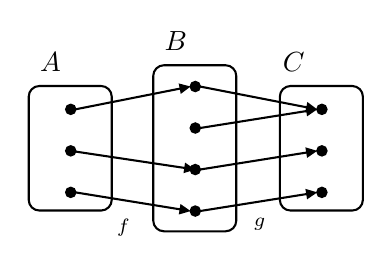
\begin{tikzpicture}[x=0.75pt,y=0.75pt,yscale=-1,xscale=1]
		%uncomment if require: \path (0,300); %set diagram left start at 0, and has height of 300
		
		%Rounded Rect [id:dp17761622576856428] 
		\draw   (90,45.14) .. controls (90,42.3) and (92.3,40) .. (95.14,40) -- (124.86,40) .. controls (127.7,40) and (130,42.3) .. (130,45.14) -- (130,94.86) .. controls (130,97.7) and (127.7,100) .. (124.86,100) -- (95.14,100) .. controls (92.3,100) and (90,97.7) .. (90,94.86) -- cycle ;
		%Rounded Rect [id:dp46557282862056737] 
		\draw   (150,35.14) .. controls (150,32.3) and (152.3,30) .. (155.14,30) -- (184.86,30) .. controls (187.7,30) and (190,32.3) .. (190,35.14) -- (190,104.86) .. controls (190,107.7) and (187.7,110) .. (184.86,110) -- (155.14,110) .. controls (152.3,110) and (150,107.7) .. (150,104.86) -- cycle ;
		%Shape: Circle [id:dp19422500705460033] 
		\draw  [fill={rgb, 255:red, 0; green, 0; blue, 0 }  ,fill opacity=1 ] (108,51.25) .. controls (108,50.01) and (109.01,49) .. (110.25,49) .. controls (111.49,49) and (112.5,50.01) .. (112.5,51.25) .. controls (112.5,52.49) and (111.49,53.5) .. (110.25,53.5) .. controls (109.01,53.5) and (108,52.49) .. (108,51.25) -- cycle ;
		%Shape: Circle [id:dp4181725904000142] 
		\draw  [fill={rgb, 255:red, 0; green, 0; blue, 0 }  ,fill opacity=1 ] (108,71.25) .. controls (108,70.01) and (109.01,69) .. (110.25,69) .. controls (111.49,69) and (112.5,70.01) .. (112.5,71.25) .. controls (112.5,72.49) and (111.49,73.5) .. (110.25,73.5) .. controls (109.01,73.5) and (108,72.49) .. (108,71.25) -- cycle ;
		%Shape: Circle [id:dp14173404339102347] 
		\draw  [fill={rgb, 255:red, 0; green, 0; blue, 0 }  ,fill opacity=1 ] (108,91.25) .. controls (108,90.01) and (109.01,89) .. (110.25,89) .. controls (111.49,89) and (112.5,90.01) .. (112.5,91.25) .. controls (112.5,92.49) and (111.49,93.5) .. (110.25,93.5) .. controls (109.01,93.5) and (108,92.49) .. (108,91.25) -- cycle ;
		%Shape: Circle [id:dp5562995636986945] 
		\draw  [fill={rgb, 255:red, 0; green, 0; blue, 0 }  ,fill opacity=1 ] (168,40.25) .. controls (168,39.01) and (169.01,38) .. (170.25,38) .. controls (171.49,38) and (172.5,39.01) .. (172.5,40.25) .. controls (172.5,41.49) and (171.49,42.5) .. (170.25,42.5) .. controls (169.01,42.5) and (168,41.49) .. (168,40.25) -- cycle ;
		%Shape: Circle [id:dp5009502155253602] 
		\draw  [fill={rgb, 255:red, 0; green, 0; blue, 0 }  ,fill opacity=1 ] (168,60.25) .. controls (168,59.01) and (169.01,58) .. (170.25,58) .. controls (171.49,58) and (172.5,59.01) .. (172.5,60.25) .. controls (172.5,61.49) and (171.49,62.5) .. (170.25,62.5) .. controls (169.01,62.5) and (168,61.49) .. (168,60.25) -- cycle ;
		%Shape: Circle [id:dp5804192548416451] 
		\draw  [fill={rgb, 255:red, 0; green, 0; blue, 0 }  ,fill opacity=1 ] (168,80.25) .. controls (168,79.01) and (169.01,78) .. (170.25,78) .. controls (171.49,78) and (172.5,79.01) .. (172.5,80.25) .. controls (172.5,81.49) and (171.49,82.5) .. (170.25,82.5) .. controls (169.01,82.5) and (168,81.49) .. (168,80.25) -- cycle ;
		%Shape: Circle [id:dp09763005580799611] 
		\draw  [fill={rgb, 255:red, 0; green, 0; blue, 0 }  ,fill opacity=1 ] (168,100.25) .. controls (168,99.01) and (169.01,98) .. (170.25,98) .. controls (171.49,98) and (172.5,99.01) .. (172.5,100.25) .. controls (172.5,101.49) and (171.49,102.5) .. (170.25,102.5) .. controls (169.01,102.5) and (168,101.49) .. (168,100.25) -- cycle ;
		%Rounded Rect [id:dp7702902675019128] 
		\draw   (211,45.14) .. controls (211,42.3) and (213.3,40) .. (216.14,40) -- (245.86,40) .. controls (248.7,40) and (251,42.3) .. (251,45.14) -- (251,94.86) .. controls (251,97.7) and (248.7,100) .. (245.86,100) -- (216.14,100) .. controls (213.3,100) and (211,97.7) .. (211,94.86) -- cycle ;
		%Shape: Circle [id:dp7132439025228492] 
		\draw  [fill={rgb, 255:red, 0; green, 0; blue, 0 }  ,fill opacity=1 ] (229,51.25) .. controls (229,50.01) and (230.01,49) .. (231.25,49) .. controls (232.49,49) and (233.5,50.01) .. (233.5,51.25) .. controls (233.5,52.49) and (232.49,53.5) .. (231.25,53.5) .. controls (230.01,53.5) and (229,52.49) .. (229,51.25) -- cycle ;
		%Shape: Circle [id:dp8656679011088042] 
		\draw  [fill={rgb, 255:red, 0; green, 0; blue, 0 }  ,fill opacity=1 ] (229,71.25) .. controls (229,70.01) and (230.01,69) .. (231.25,69) .. controls (232.49,69) and (233.5,70.01) .. (233.5,71.25) .. controls (233.5,72.49) and (232.49,73.5) .. (231.25,73.5) .. controls (230.01,73.5) and (229,72.49) .. (229,71.25) -- cycle ;
		%Shape: Circle [id:dp3810099412269634] 
		\draw  [fill={rgb, 255:red, 0; green, 0; blue, 0 }  ,fill opacity=1 ] (229,91.25) .. controls (229,90.01) and (230.01,89) .. (231.25,89) .. controls (232.49,89) and (233.5,90.01) .. (233.5,91.25) .. controls (233.5,92.49) and (232.49,93.5) .. (231.25,93.5) .. controls (230.01,93.5) and (229,92.49) .. (229,91.25) -- cycle ;
		%Straight Lines [id:da5744148941789291] 
		\draw    (112.5,51.25) -- (165.06,40.83) ;
		\draw [shift={(168,40.25)}, rotate = 168.79] [fill={rgb, 255:red, 0; green, 0; blue, 0 }  ][line width=0.08]  [draw opacity=0] (5.36,-2.57) -- (0,0) -- (5.36,2.57) -- cycle    ;
		%Straight Lines [id:da19500736197062674] 
		\draw    (110.25,71.25) -- (167.28,79.8) ;
		\draw [shift={(170.25,80.25)}, rotate = 188.53] [fill={rgb, 255:red, 0; green, 0; blue, 0 }  ][line width=0.08]  [draw opacity=0] (5.36,-2.57) -- (0,0) -- (5.36,2.57) -- cycle    ;
		%Straight Lines [id:da16617365221937108] 
		\draw    (112.5,91.25) -- (165.04,99.77) ;
		\draw [shift={(168,100.25)}, rotate = 189.21] [fill={rgb, 255:red, 0; green, 0; blue, 0 }  ][line width=0.08]  [draw opacity=0] (5.36,-2.57) -- (0,0) -- (5.36,2.57) -- cycle    ;
		%Straight Lines [id:da3123797973376088] 
		\draw    (172.5,40.25) -- (226.06,50.68) ;
		\draw [shift={(229,51.25)}, rotate = 191.02] [fill={rgb, 255:red, 0; green, 0; blue, 0 }  ][line width=0.08]  [draw opacity=0] (5.36,-2.57) -- (0,0) -- (5.36,2.57) -- cycle    ;
		%Straight Lines [id:da4140086921793451] 
		\draw    (172.5,60.25) -- (226.04,51.72) ;
		\draw [shift={(229,51.25)}, rotate = 170.95] [fill={rgb, 255:red, 0; green, 0; blue, 0 }  ][line width=0.08]  [draw opacity=0] (5.36,-2.57) -- (0,0) -- (5.36,2.57) -- cycle    ;
		%Straight Lines [id:da1446468918418573] 
		\draw    (172.5,80.25) -- (226.04,71.72) ;
		\draw [shift={(229,71.25)}, rotate = 170.95] [fill={rgb, 255:red, 0; green, 0; blue, 0 }  ][line width=0.08]  [draw opacity=0] (5.36,-2.57) -- (0,0) -- (5.36,2.57) -- cycle    ;
		%Straight Lines [id:da47355823667796293] 
		\draw    (172.5,100.25) -- (226.04,91.72) ;
		\draw [shift={(229,91.25)}, rotate = 170.95] [fill={rgb, 255:red, 0; green, 0; blue, 0 }  ][line width=0.08]  [draw opacity=0] (5.36,-2.57) -- (0,0) -- (5.36,2.57) -- cycle    ;
		
		% Text Node
		\draw (131,102.4) node [anchor=north west][inner sep=0.75pt]  [font=\scriptsize]  {$f$};
		% Text Node
		\draw (197,102.4) node [anchor=north west][inner sep=0.75pt]  [font=\scriptsize]  {$g$};
		% Text Node
		\draw (94,22.4) node [anchor=north west][inner sep=0.75pt]    {$A$};
		% Text Node
		\draw (154,12.4) node [anchor=north west][inner sep=0.75pt]    {$B$};
		% Text Node
		\draw (211,22.4) node [anchor=north west][inner sep=0.75pt]    {$C$};
		
		
	\end{tikzpicture}
\end{figure}

